\documentclass[xcolor=dvipsnames, USenglish]{beamer}  %notes=show to print them in the generated pdf
% Packages for a reasonable beamer session
\usepackage[T1]{fontenc}
%\usepackage[ansinew]{inputenc}
\usepackage[utf8]{inputenc}
\usepackage{textcomp}
\usepackage{lmodern}
\usepackage{csquotes}
\usepackage[english]{babel}
%\usepackage{babel}

\usepackage{graphicx}

\usepackage{amsmath}
\usepackage{amsfonts}
\usepackage{amssymb}
\usepackage{amsthm}
\usepackage{bm}

\usepackage{booktabs}
\usepackage{tabularx}

\usepackage{hyperref}

\usepackage{ellipsis}

% Additional packages
\usepackage{graphicx}
\usepackage{subfigure}
\usepackage{xcolor}
\usepackage{minted}

\usepackage[style=authoryear, backend=biber]{biblatex}
\setbeamertemplate{itemize/enumerate body begin}{\setlength{\leftmargini}{1.5em}}
\renewcommand*{\nameyeardelim}{\addcomma\addspace}
\addbibresource{\jobname.bib}
\renewcommand{\footnotesize}{\tiny}

\usepackage{tikz,pgf,calc}
%\usetikzlibrary{matrix, shapes, positioning, calc,
%  decorations.pathreplacing, shapes.geometric, arrows}
\usetikzlibrary{shapes.geometric, arrows, calc}
\tikzstyle{startstop} = [rectangle, rounded corners, minimum width=3cm, minimum height=1cm, text centered, text width=1.5cm, draw=black, fill=red!30]
\tikzstyle{io} = [trapezium, trapezium left angle=70, trapezium right angle=110, minimum width=3cm, minimum height=1cm, text centered, draw=black, fill=blue!30]
\tikzstyle{process} = [rectangle, minimum width=3cm, minimum height=1cm, text centered, draw=black, fill=orange!30]
\tikzstyle{decision} = [diamond, minimum width=3cm, minimum height=0.5cm, text centered, draw=black, fill=green!30]
\tikzstyle{arrow} = [thick,->,>=stealth]

%% References
\newlength\leftsidebar
\makeatletter
\setlength\leftsidebar{\beamer@leftsidebar}
\makeatother

\usepackage[absolute,overlay]{textpos}
\newenvironment{reference}[2]{%
  \begin{textblock*}{\textwidth}(\leftsidebar+#1,\paperheight-#2)
      \scriptsize\bgroup\color{red!50!black}}{\egroup\end{textblock*}}

% Path to graphics
\graphicspath{{../img/}}

% Sources
\usepackage{setspace}
\newcommand{\source}[1]{\begin{spacing}{0.5}{\fontsize{5}{6}\selectfont source: \itshape {#1}}\end{spacing}}
 % PACKAGES
% Collection of useful mathematical symbols and commands
% Calculus
\newcommand{\ud}{\mathrm{d}}
\newcommand{\pder}[2]{\frac{\partial{#1}}{\partial{#2}}}
\newcommand{\dpder}[2]{\frac{\partial^2{#1}}{\partial{#2^2}}}
\newcommand{\sderp}[3]{\frac{\partial^2{#1}}{\partial{#2}\partial{#3}}}
\newcommand{\tder}[2]{\frac{\ud{#1}}{\ud{#2}}}
\newcommand{\rot}[1]{\nabla \times {#1}}
\newcommand{\diver}[1]{\nabla \cdot {#1}}
\newcommand{\definter}[4]{\int_{#1}^{#2} {#3}\ud {#4}}
\newcommand{\inter}[2]{\int {#1}\ud {#2}}
\newcommand{\braket}[2]{\langle {#1} , {#2} \rangle}
% Misc
\newcommand{\eval}[1]{\Big |_{#1}}
\newcommand{\bset}[1]{\big\lbrace {#1} \big\rbrace}
\newcommand{\stimes}[2]{{#1}\!\times\!{#2}}
\newcommand{\trp}{\top}
\newcommand{\preup}[2]{{}^{#2}\!{#1}}

% Operators
\DeclareMathOperator*{\armin}{arg\,min}
\DeclareMathOperator*{\armax}{arg\,max}
\DeclareMathOperator*{\rank}{rank}
\DeclareMathOperator*{\cov}{cov}
\DeclareMathOperator*{\nullsp}{null}
% Logicals
\newcommand{\suchthat}{\big \backslash \;}
   % SYMBOLS

% ----------- extra packages
\usepackage{beamer_themes/beamerthemeEawag_blue} % Eawag style

% ----------- Extra symbols
\newcommand{\ccov}[1]{{\color{red}k}\left(#1\right)}
\newcommand{\cmean}[1]{{\color{blue}m}\left(#1\right)}
\newcommand{\sm}{\scalebox{0.5}{-1}}

% ----------- For boxed equations
\usepackage{amsmath}
\usepackage{empheq}
\usepackage[most]{tcolorbox}
\usepackage{siunitx}

\newtcbox{\mymath}[1][]{%
    nobeforeafter, math upper, tcbox raise base,
    enhanced, colframe=blue!30!black,
    colback=blue!30, boxrule=1pt,
    #1}



%----------------
% title information
\title{\centerline{Fast early flood warning systems}\\ \centerline{exploiting catchment specific behavior}}
\author[\texttt{\underline{S. Rusca}, J. P. Carbajal}]{\underline{Sebastiano Rusca}, Juan Pablo Carbajal}
\institute[Eawag]{Eawag: Swiss Federal Institute of Aquatic Science
  and Technology}
\date[14.06.2018]{June 14, 2018}


\begin{document}
%%%%%%%%%%%%%%%%%%%%%%%%%%%%%%%%%%%%%%%%%%%%%%%%%%%%%%%%%%%%%%%%%%%%%%%%%%%%%%%%
% TITLE SLIDE
\setbeamertemplate{background}{
  
\includegraphics[width=\paperwidth,height=\paperheight]
  {beamer_themes/background_title_IAHR.png}}

{
\setbeamertemplate{footline}{}
  \begin{frame}
    \titlepage
  \end{frame}
}

\setbeamertemplate{background}{

\includegraphics[width=\paperwidth,height=\paperheight]
{beamer_themes/background_slides_blue.png}}
\setbeamertemplate{footline}[Sebastiano Rusca]
\addtocounter{framenumber}{-1}

% * Hello everybody, I am Sebastiano Rusca, Master student in environmental 
%   engineering of the ETH Zurich
% * I am gonna present a part of my master thesis, which I carried out at the 
%   eawag, the Swiss federal institute of aquatic science and technology, under
%   the supervision of Juan Pablo Carbajal
% * The title of my presentation is "Fast early flood warning systems 
%   exploiting catchment specific behavior", so let's have a look what this is 
%   all about

%%%%%%%%%%%%%%%%%%%%%%%%%%%%%%%%%%%%%%%%%%%%%%%%%%%%%%%%%%%%%%%%%%%%%%%%%%%%%%%%
% INTRODUCTION
\section{Introduction}
  \begin{frame}
    \frametitle{General framework}
    \centering
    \begin{minipage}{.48\textwidth}
      \hfill
      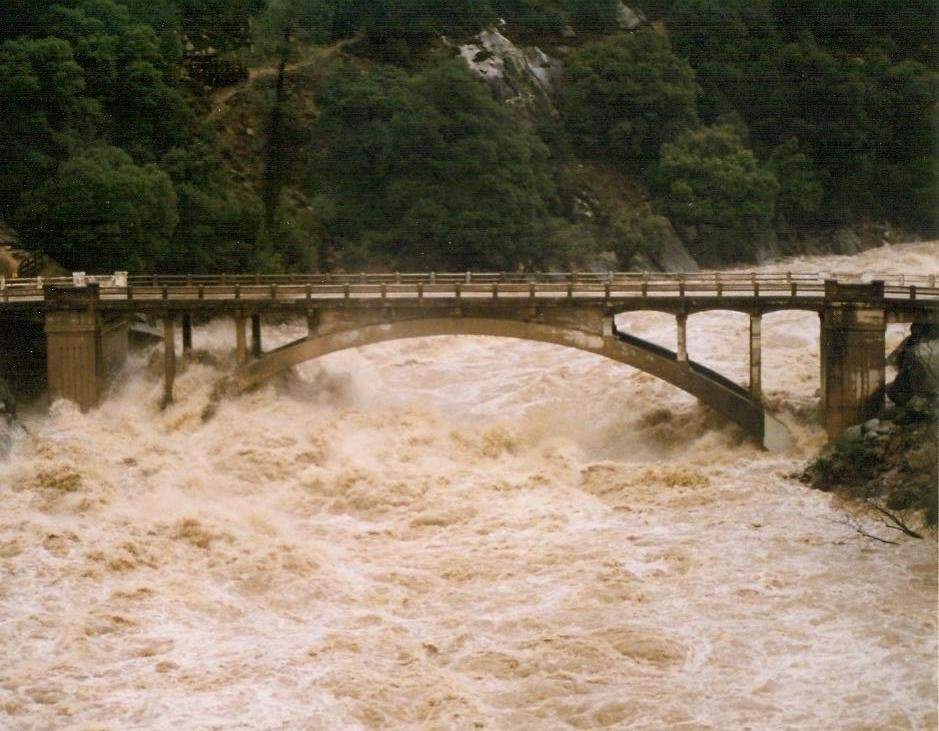
\includegraphics[width=0.7\textwidth]{img/flood_bridge.jpg}
      \raggedright\source{https://www.geocaching.com/geocache/GC4T07C\_hwy-49-crossing-1921?guid=6b2187dd-2cf0-4ce3-880c-70a6cc544114}
    \end{minipage}
    %
    \begin{minipage}{.48\textwidth}
      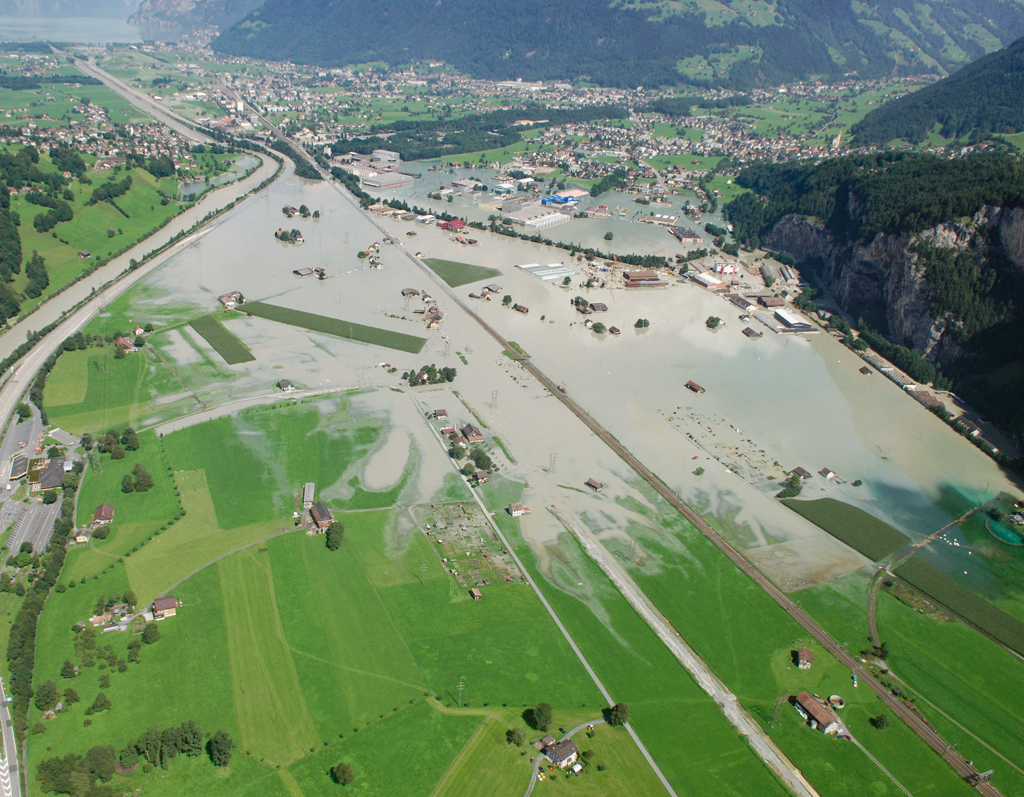
\includegraphics[width=0.7\textwidth]{img/flooding.jpg}
      \hfill
      \raggedright\source{https://www.espazium.ch/entschrftes-risiko-auf-nordsdachse}
    \end{minipage}
    \\
    \begin{minipage}{.48\textwidth}
      \hfill
      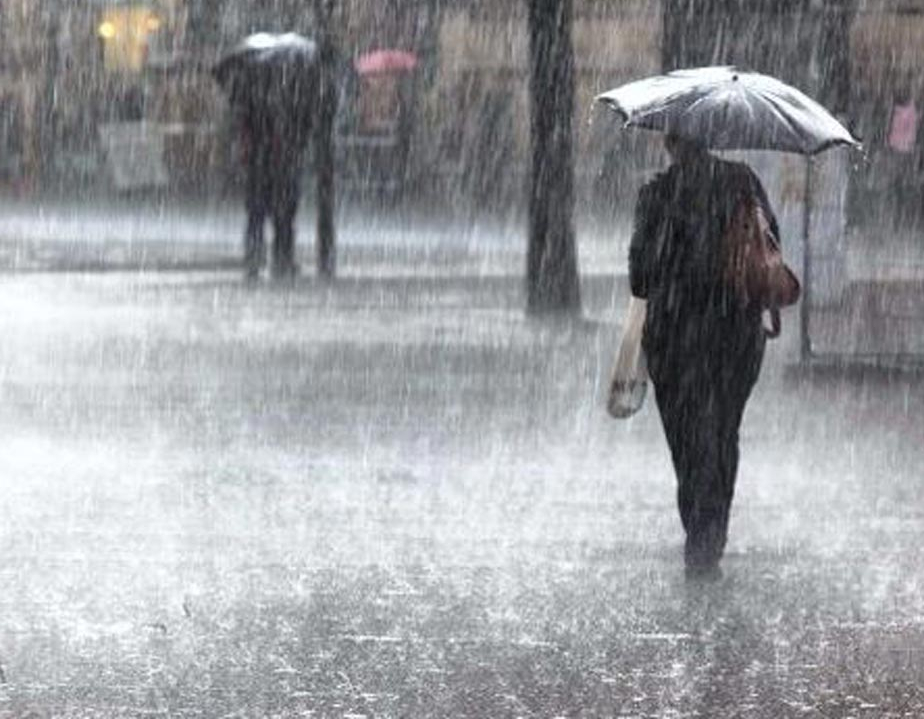
\includegraphics[width=0.7\textwidth]{img/heavy_rainfall.jpg}
      \raggedright\source{https://guardian.ng/news/heavy-rainfall-cuts-off-kuje-community}
    \end{minipage}
    %
    \begin{minipage}{.48\textwidth}
      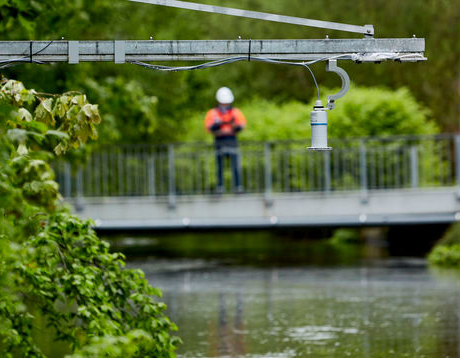
\includegraphics[width=0.7\textwidth]{img/radar_measurement.jpg}
      \hfill
      \raggedright\source{https://www.endress.com/en/Field-instruments-overview/level-measurement/Radar-Micropilot-FMR10}
    \end{minipage}
  \end{frame}

% * Floods represent one of the major socio-economic risks for the population
% * For this reason, the interest in being able to effectively predict them
%   has become a hot topic
% * Real time discharge and water depth monitoring brought a big contribution to
%   the prediction of floods, allowing for the implementation of automatic
%   systems sounding an alarm as soon as a certain threshold is reached
% * Such systems can be coupled with rainfall-runoff models, able to predict
%   flooding based on meteorological data
%   However, such models are often quite expensive to evaluate, with runs which
%   can take up to several hours
% * This doesn't allow for near-real time predictions nor for continuous
%   evaluation of the model to take account of the time evolution
% * We present here a machine learning based model exploiting the catchment
%   specific behavior to develop an efficient surrogate model computing the
%   time-to-threshold, the time elapsed from the beginning of a rain event to
%   the moment when a certain threshold discharge at a given point is reached. 
%   This discharge is the one at which flooding starts.
% * To produce the needed datasets simulation with a simulator solving the 
%   shallow water equation were performed

%%%%%%%%%%%%%%%%%%%%%%%%%%%%%%%%%%%%%%%%%%%%%%%%%%%%%%%%%%%%%%%%%%%%%%%%%%%%%%%%
% SIMULATION SET-UP
\section{Methodology}
  \begin{frame}
    \frametitle{Simulations set-up}
    \centering
    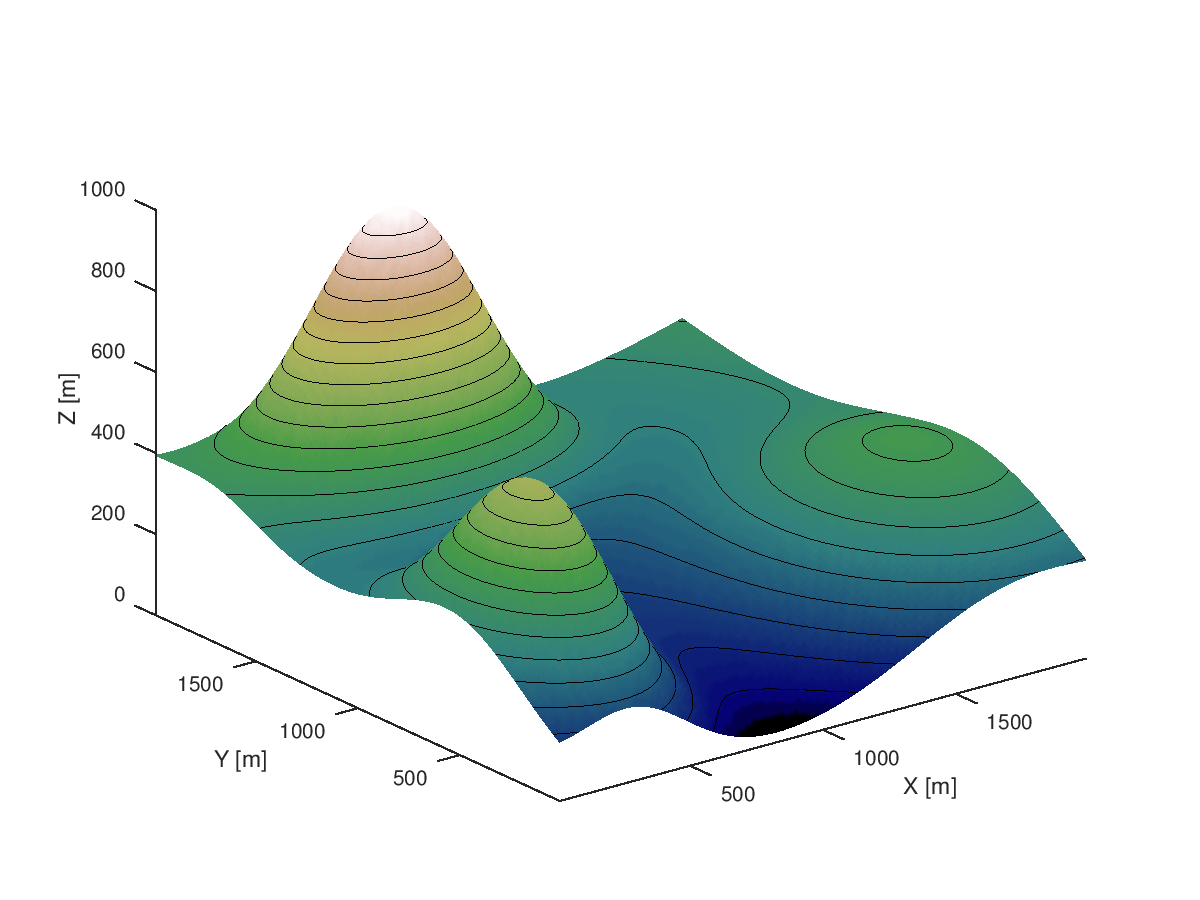
\includegraphics[width=0.7\textwidth]{img/topography.png}
    \inputminted[fontsize=\scriptsize,
                firstline=6,
                lastline=9,
                numbersep=2pt,
                gobble=0,
                frame=lines,
                bgcolor=bg,
                framesep=2mm]{octave}
                {code.m}
  \end{frame}

% * The synthetic topography that you see here was produced with "Octave" and was
%   used for running all simulations
% * It represents a catchment of 2 x 2 km crossed by a channel conveying the water
%   and taking it out of the domain through the lower boundary
% * We used a synthetic topography because of its smoothness. This way we can use
%   a coarse resolutions without losing relevant features
% * We ran 50 simulations, all representing different rain events:
% * Every rain event is characterized by a different rain intensity and a
%   different initial soil saturation
% * The rain was uniformly and constantly applied to the topography during 6 hours
% * The values used for the initial soil saturations are also uniformly
%   distributed over the catchment
% * The simulation duration was set to 9 hours in order to observe the behavior
%   after the rain has stopped

%%%%%%%%%%%%%%%%%%%%%%%%%%%%%%%%%%%%%%%%%%%%%%%%%%%%%%%%%%%%%%%%%%%%%%%%%%%%%%%%
% SIMULATION RESULTS
  \begin{frame}
    \frametitle{Simulations results}
    \centering    
    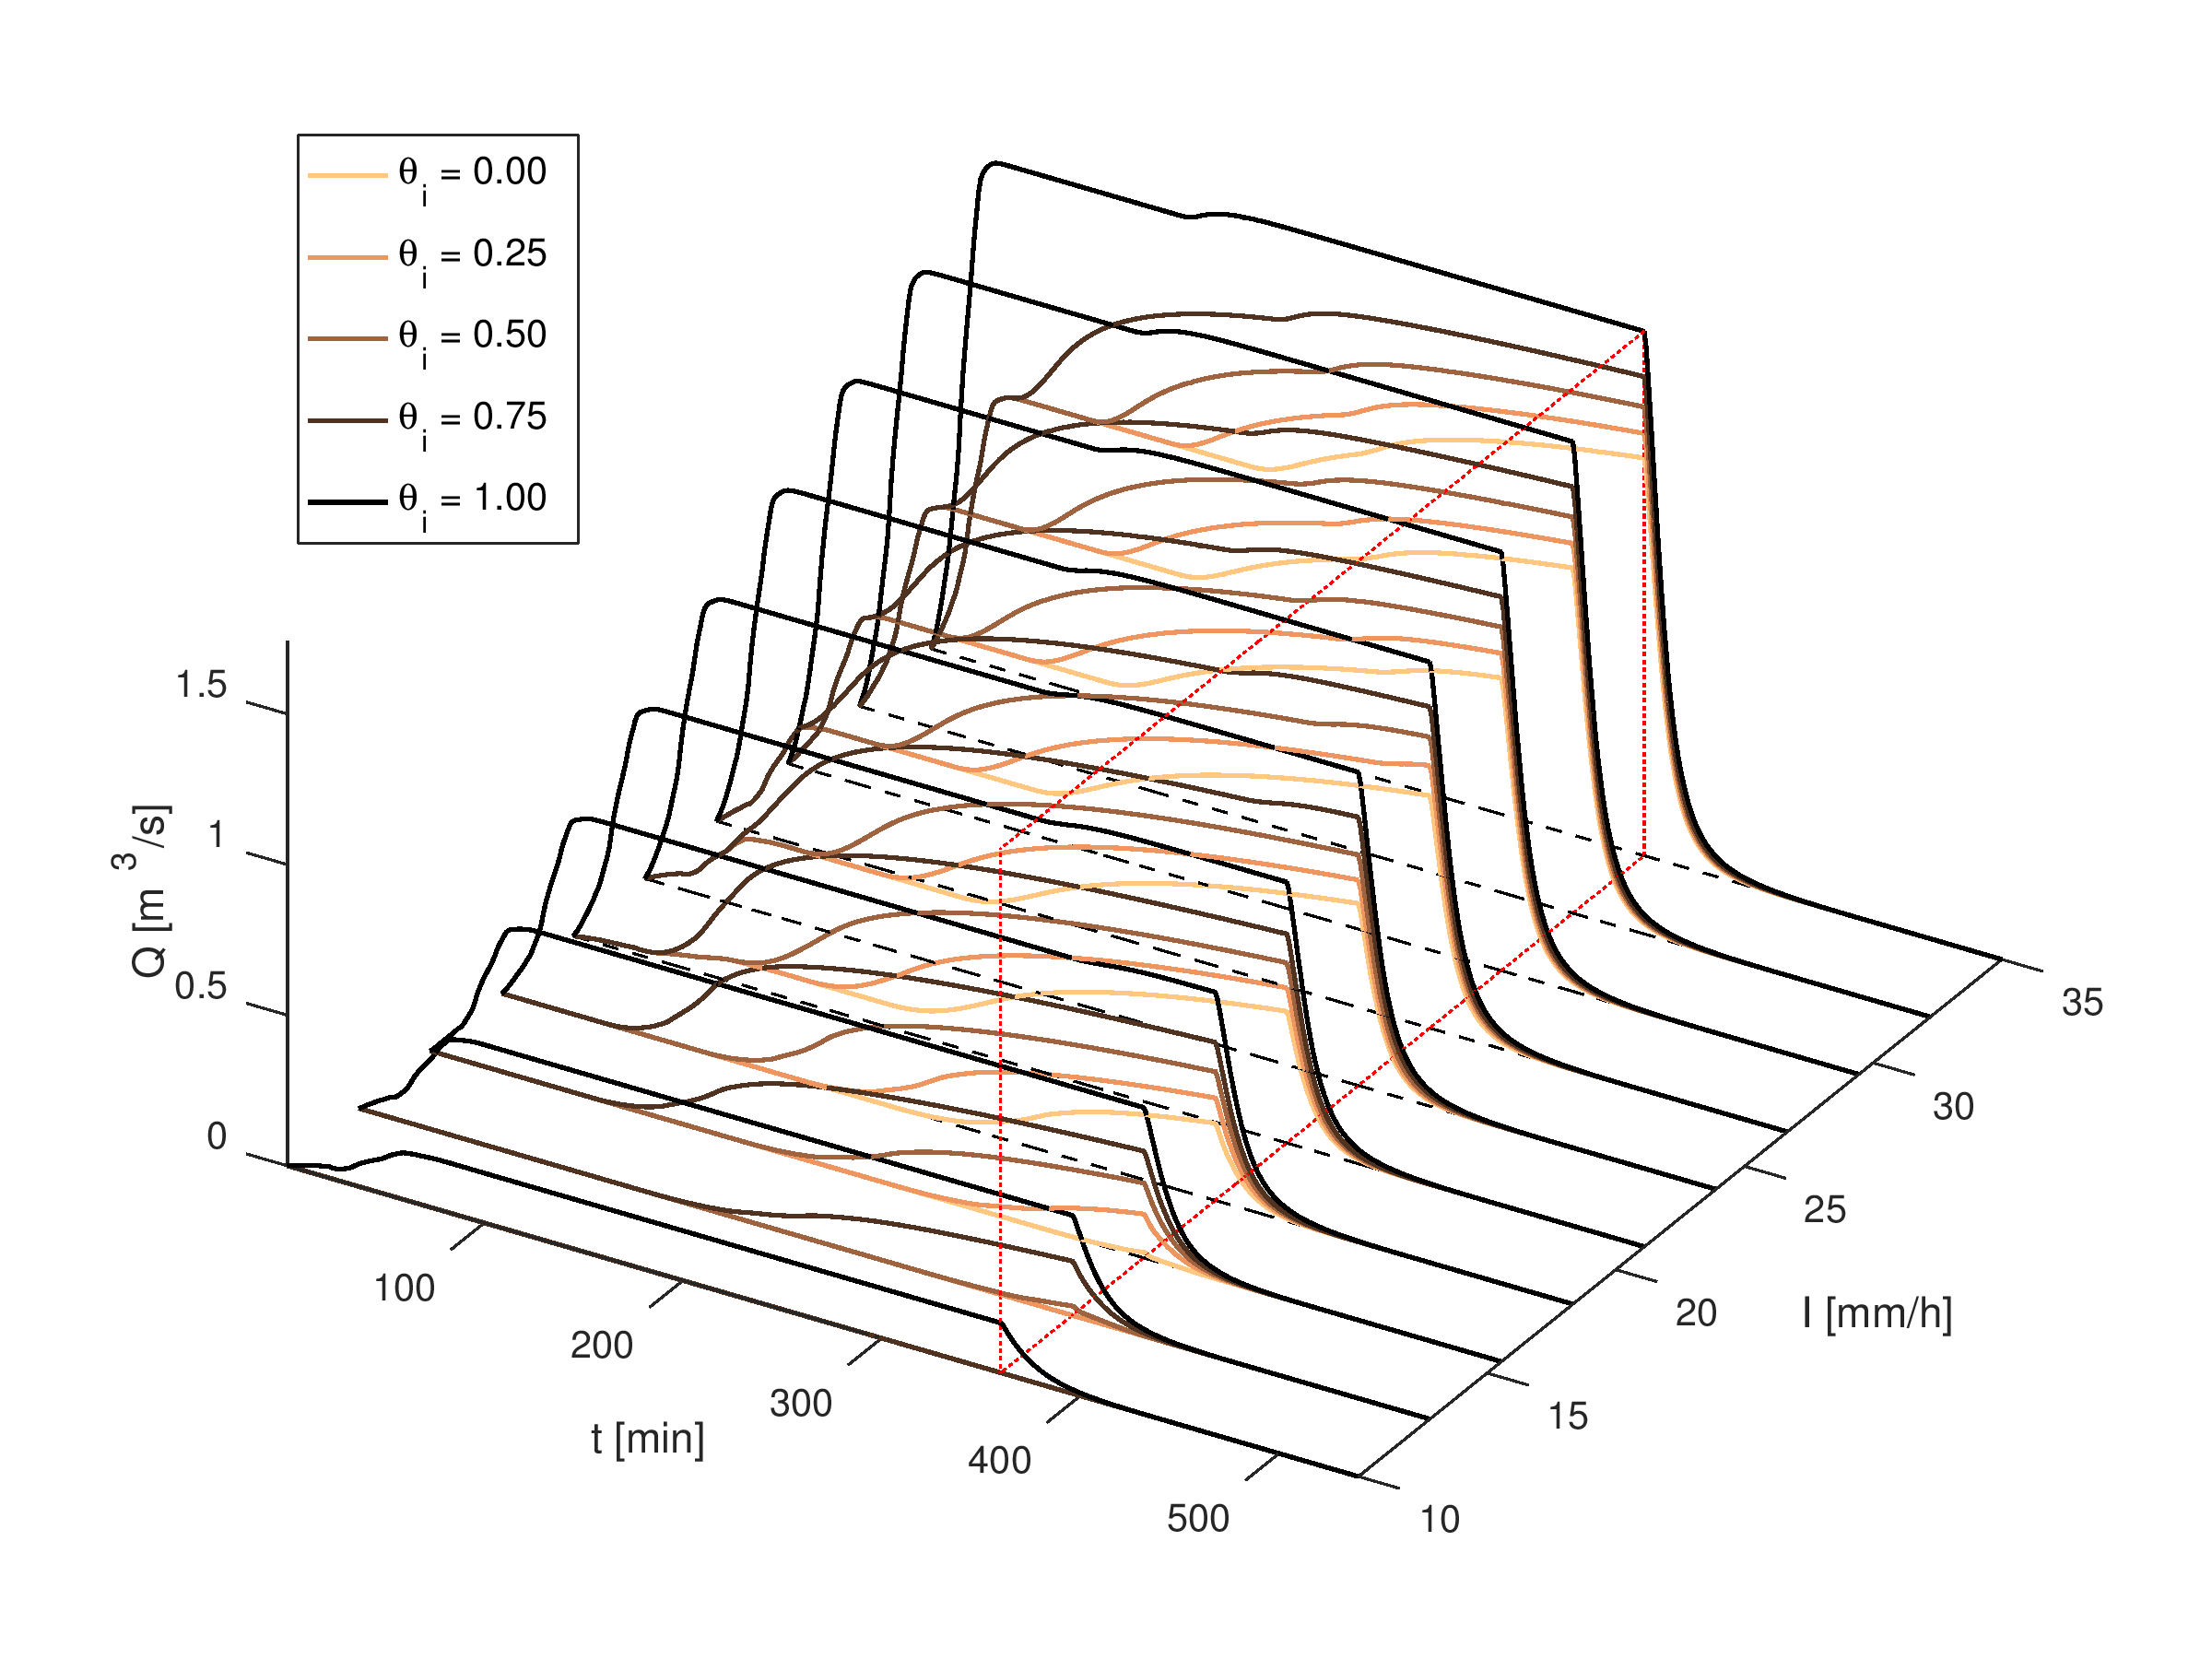
\includegraphics[width=0.8\textwidth]{img/hydrographs3d.png}
  \end{frame}

% * From the simulations we extracted the discharge at the channel outlet
% * This plot represents the hydrographs obtained for the 50 simulations
% * Rain intensity is plotted on the y-axis and for initial saturation a color
%   scale is used
% * The red frame represents the end of the rain events
% * We can notice that some rain events produced absolutely no channel discharge
%   while those with high initial soil saturation reached their peak discharge
%   very fast
% * Many hydrographs show an interesting behavior: a first plateau after some
%   time, followed by one or two bumps
% * Let's take a closer look at one of these hydrographs

%%%%%%%%%%%%%%%%%%%%%%%%%%%%%%%%%%%%%%%%%%%%%%%%%%%%%%%%%%%%%%%%%%%%%%%%%%%%%%%%
% DISCONTINUITY TIME TO THRESHOLD
  \begin{frame}
    \frametitle{Dataset extraction}
    \centering
    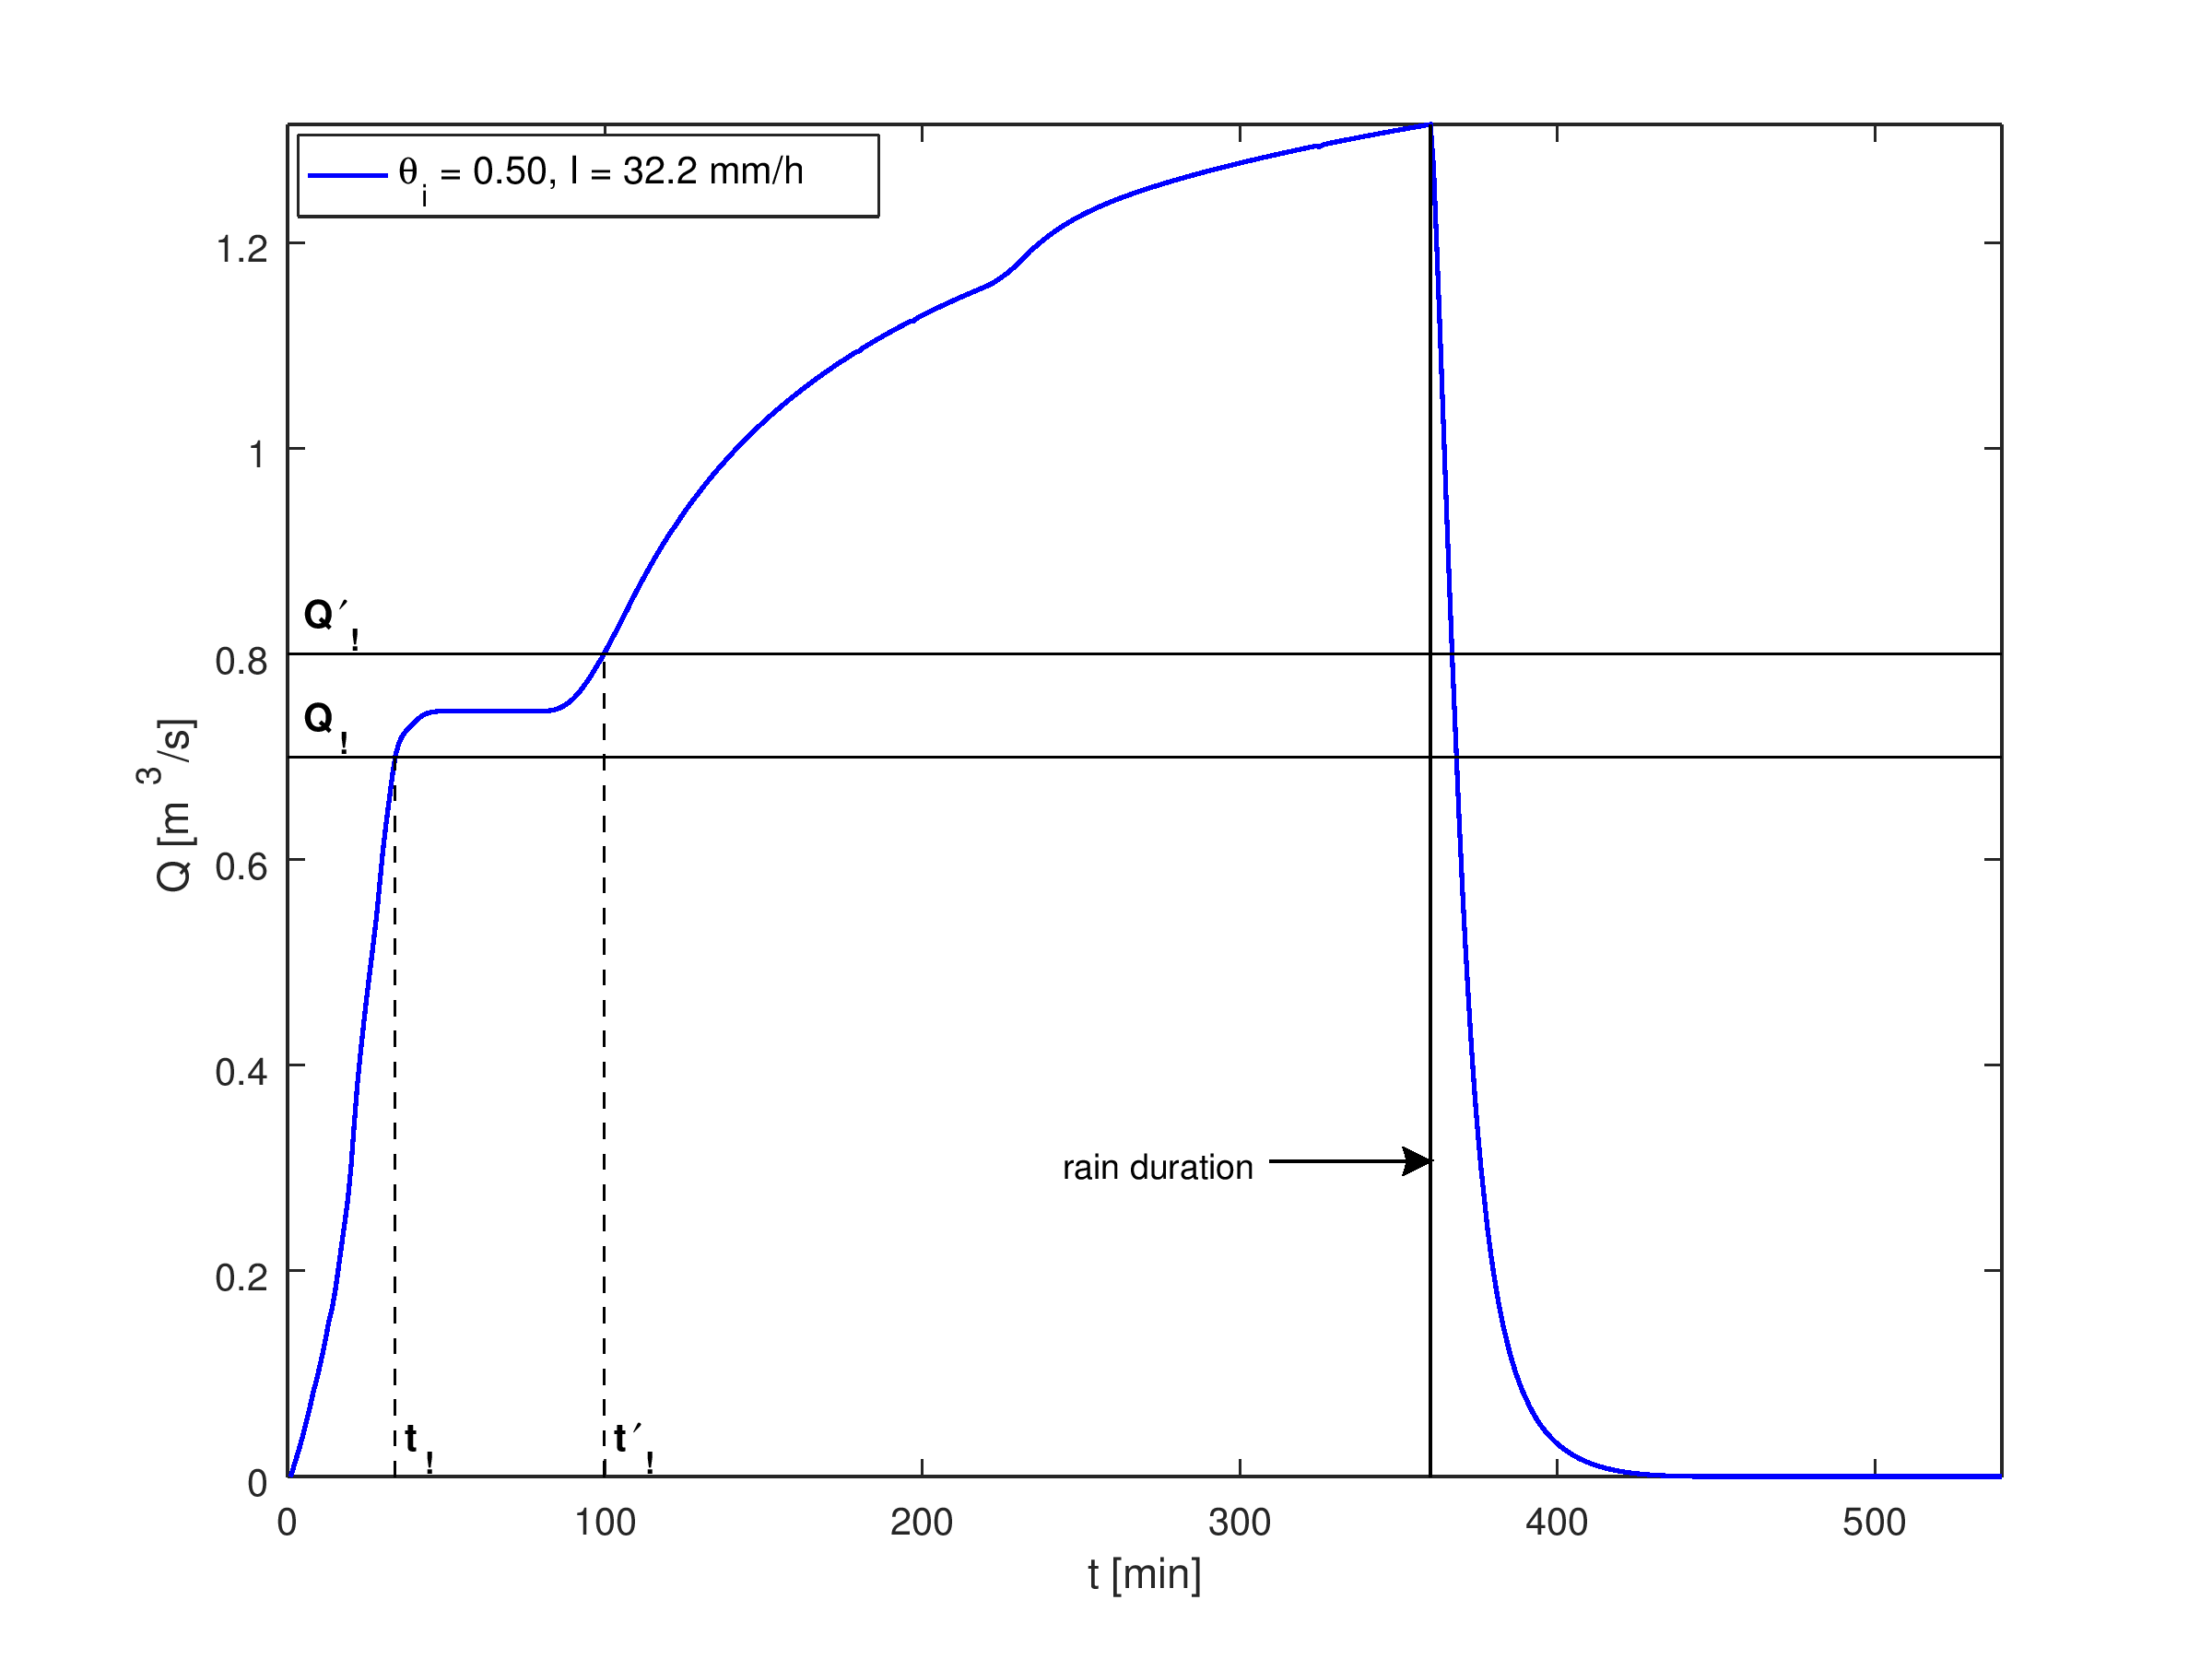
\includegraphics[width=0.8\textwidth]{img/hydrograph.png}
  \end{frame}

% * Here we better see this plateau and the following bumps
% * These can be explained by the fact that water coming down from the
%   "mountains" travels faster than that from the flat areas, generating
%   different arrival waves
% * For the chosen task we need to set a threshold discharge
% * We can notice that the threshold chosen plays a major role in the resulting
%   time-to-threshold
% * In this region moving the threshold very little causes an abrupt variations of
%   the resulting time to threshold
% * The time to threshold is therefore a discontinuous quantity, which makes it
%   challenging to predict
% * For this reason after we fixed a threshold we decided to separate the
%   task in two parts

%%%%%%%%%%%%%%%%%%%%%%%%%%%%%%%%%%%%%%%%%%%%%%%%%%%%%%%%%%%%%%%%%%%%%%%%%%%%%%%%
% CLASSIFY THE RAIN EVENTS
\section{Results}
  \begin{frame}
    \frametitle{Rain events classification}
    \centering
    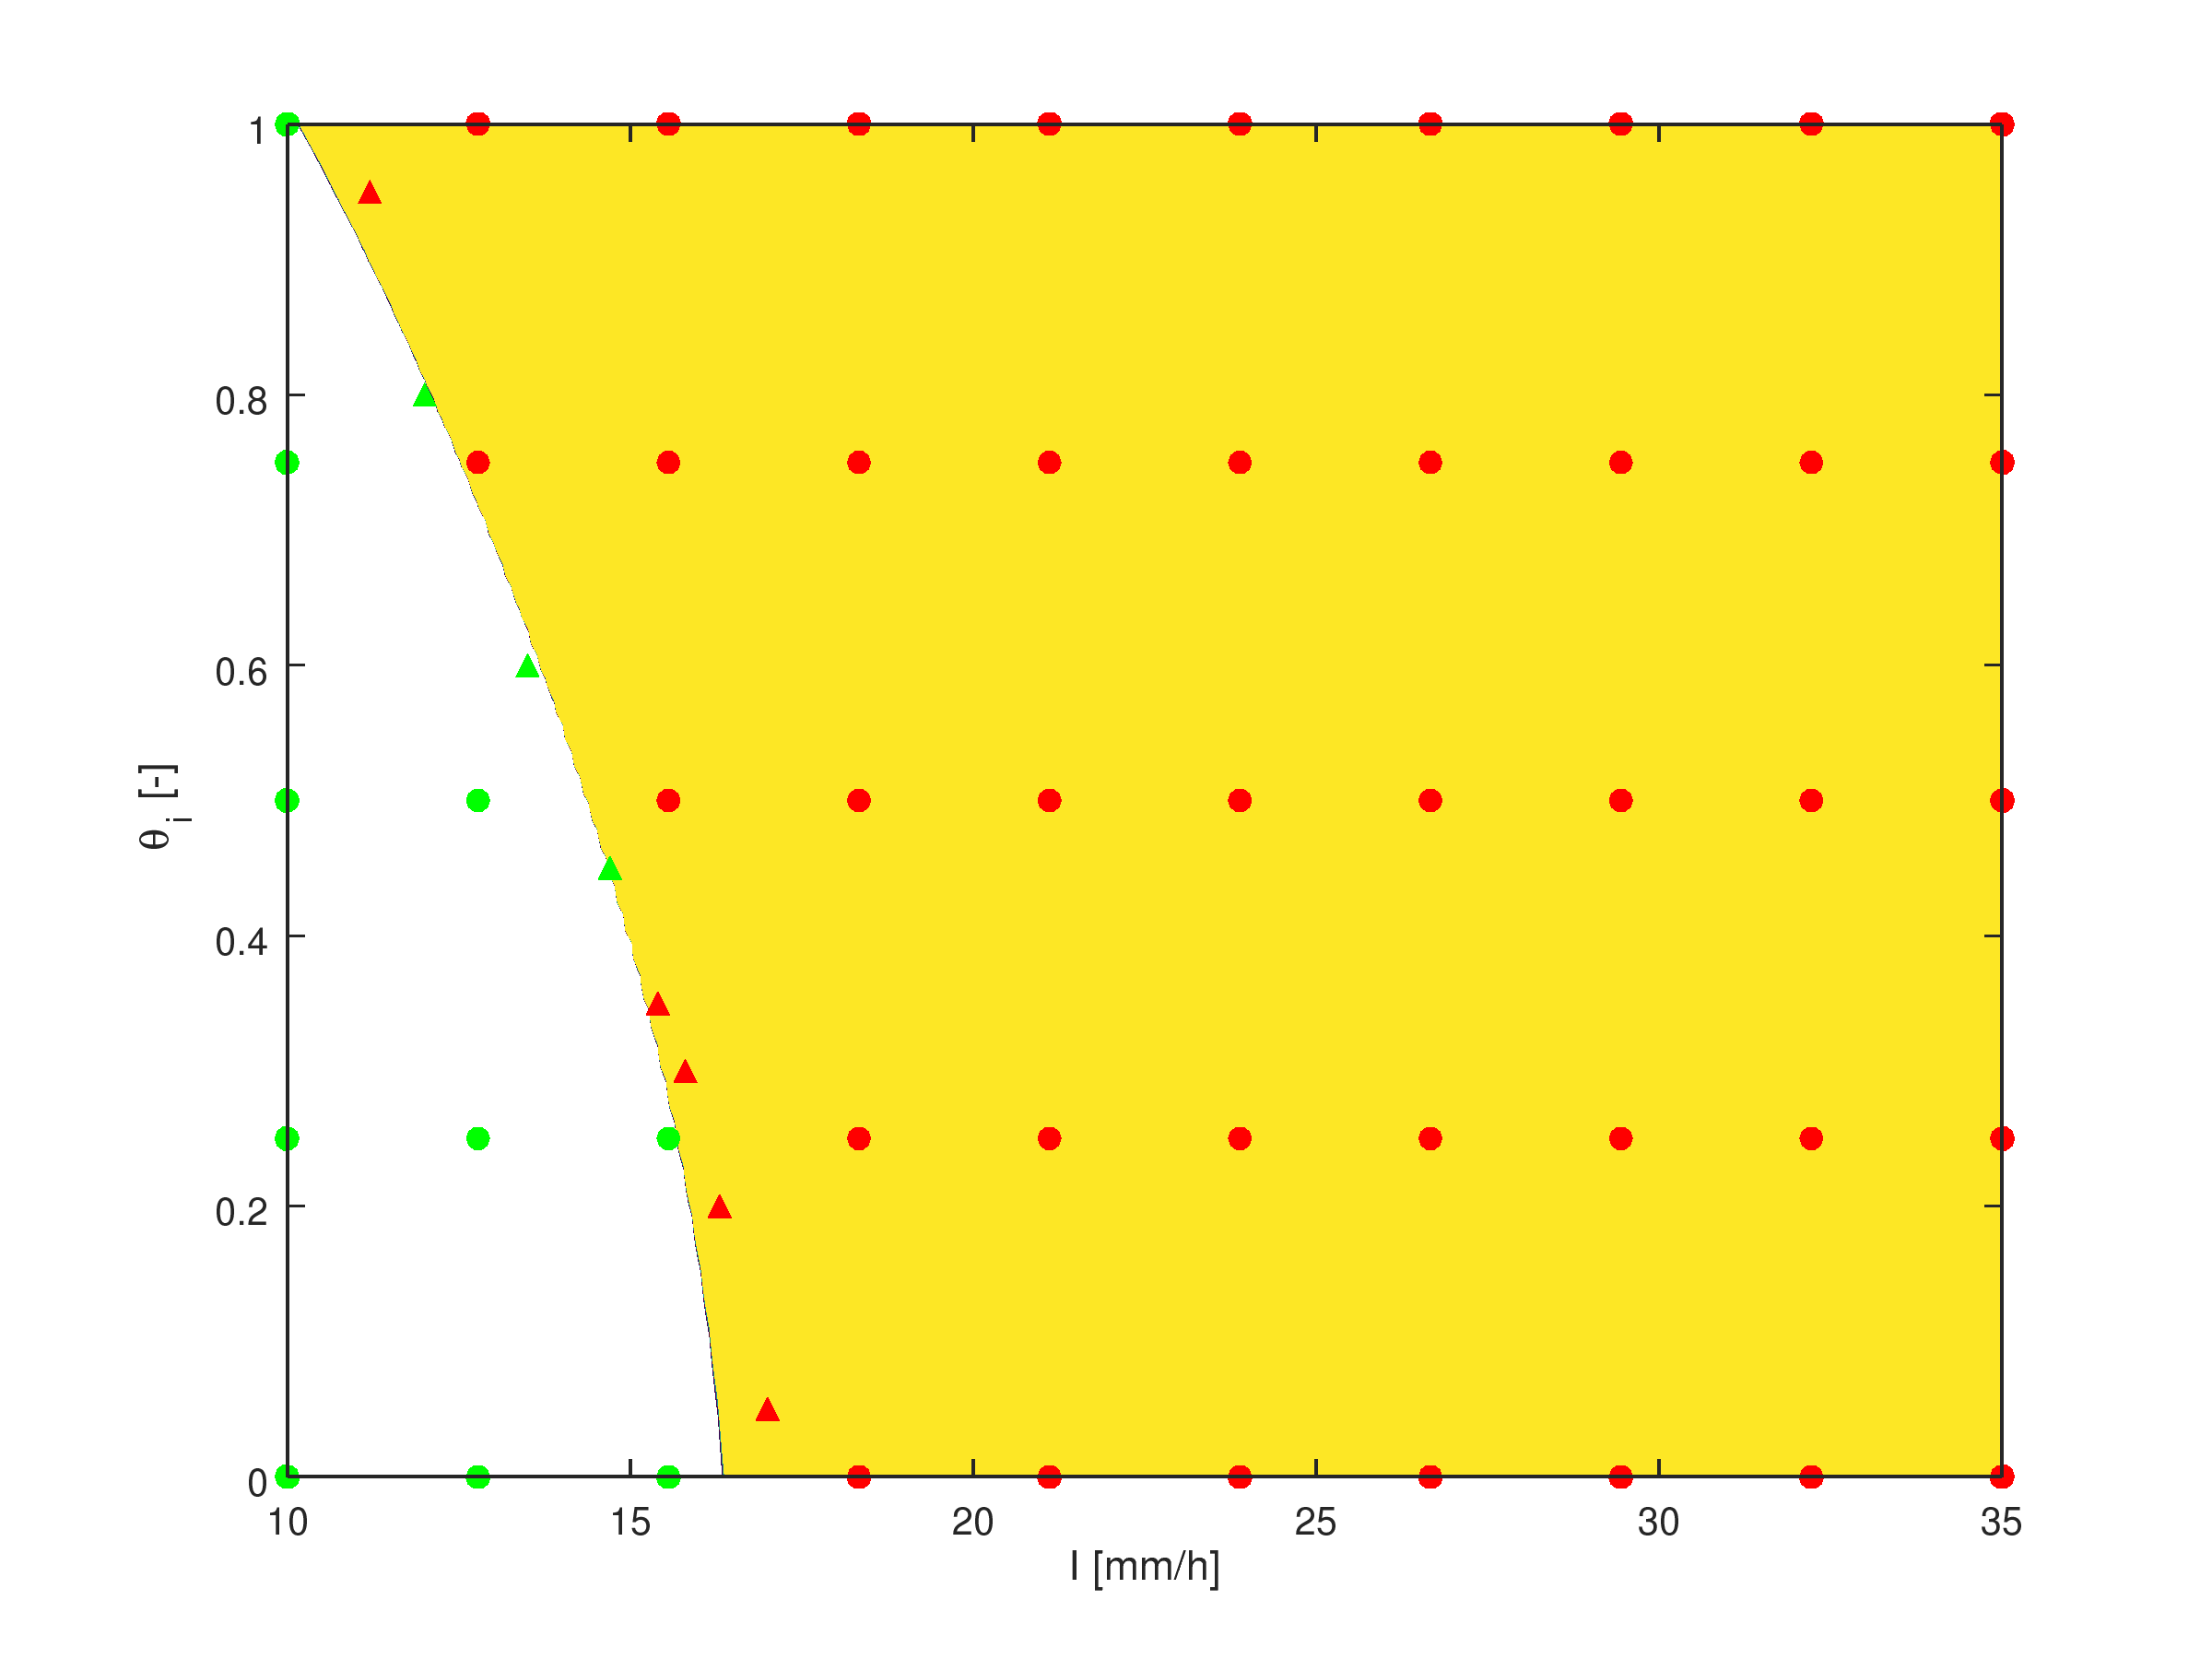
\includegraphics[width=0.8\textwidth]{img/classifier.png}
  \end{frame}

% * In this first part we classified the rain events
% * The points on the plot represent the different rain events, characterized by
%   different combinations of rain intensity and initial soil saturation
% * The red ones are those where the threshold was exceeded, while the green
%   ones are those were it wasn't
% * A Gaussian process based classifier was used to perform the classification
% * The yellow region is the one separating points exceeding the
%   threshold from those not exceeding the threshold
% * Only the points exceeding the threshold were then used to compute the 
%   time-to-threshold

%%%%%%%%%%%%%%%%%%%%%%%%%%%%%%%%%%%%%%%%%%%%%%%%%%%%%%%%%%%%%%%%%%%%%%%%%%%%%%%%
% COMPUTING THE TIME-TO-THRESHOLD
\section{Results}
  \begin{frame}
    \frametitle{Predicting the \emph{time-to-threshold}}
    \only<1>{
    \centering
    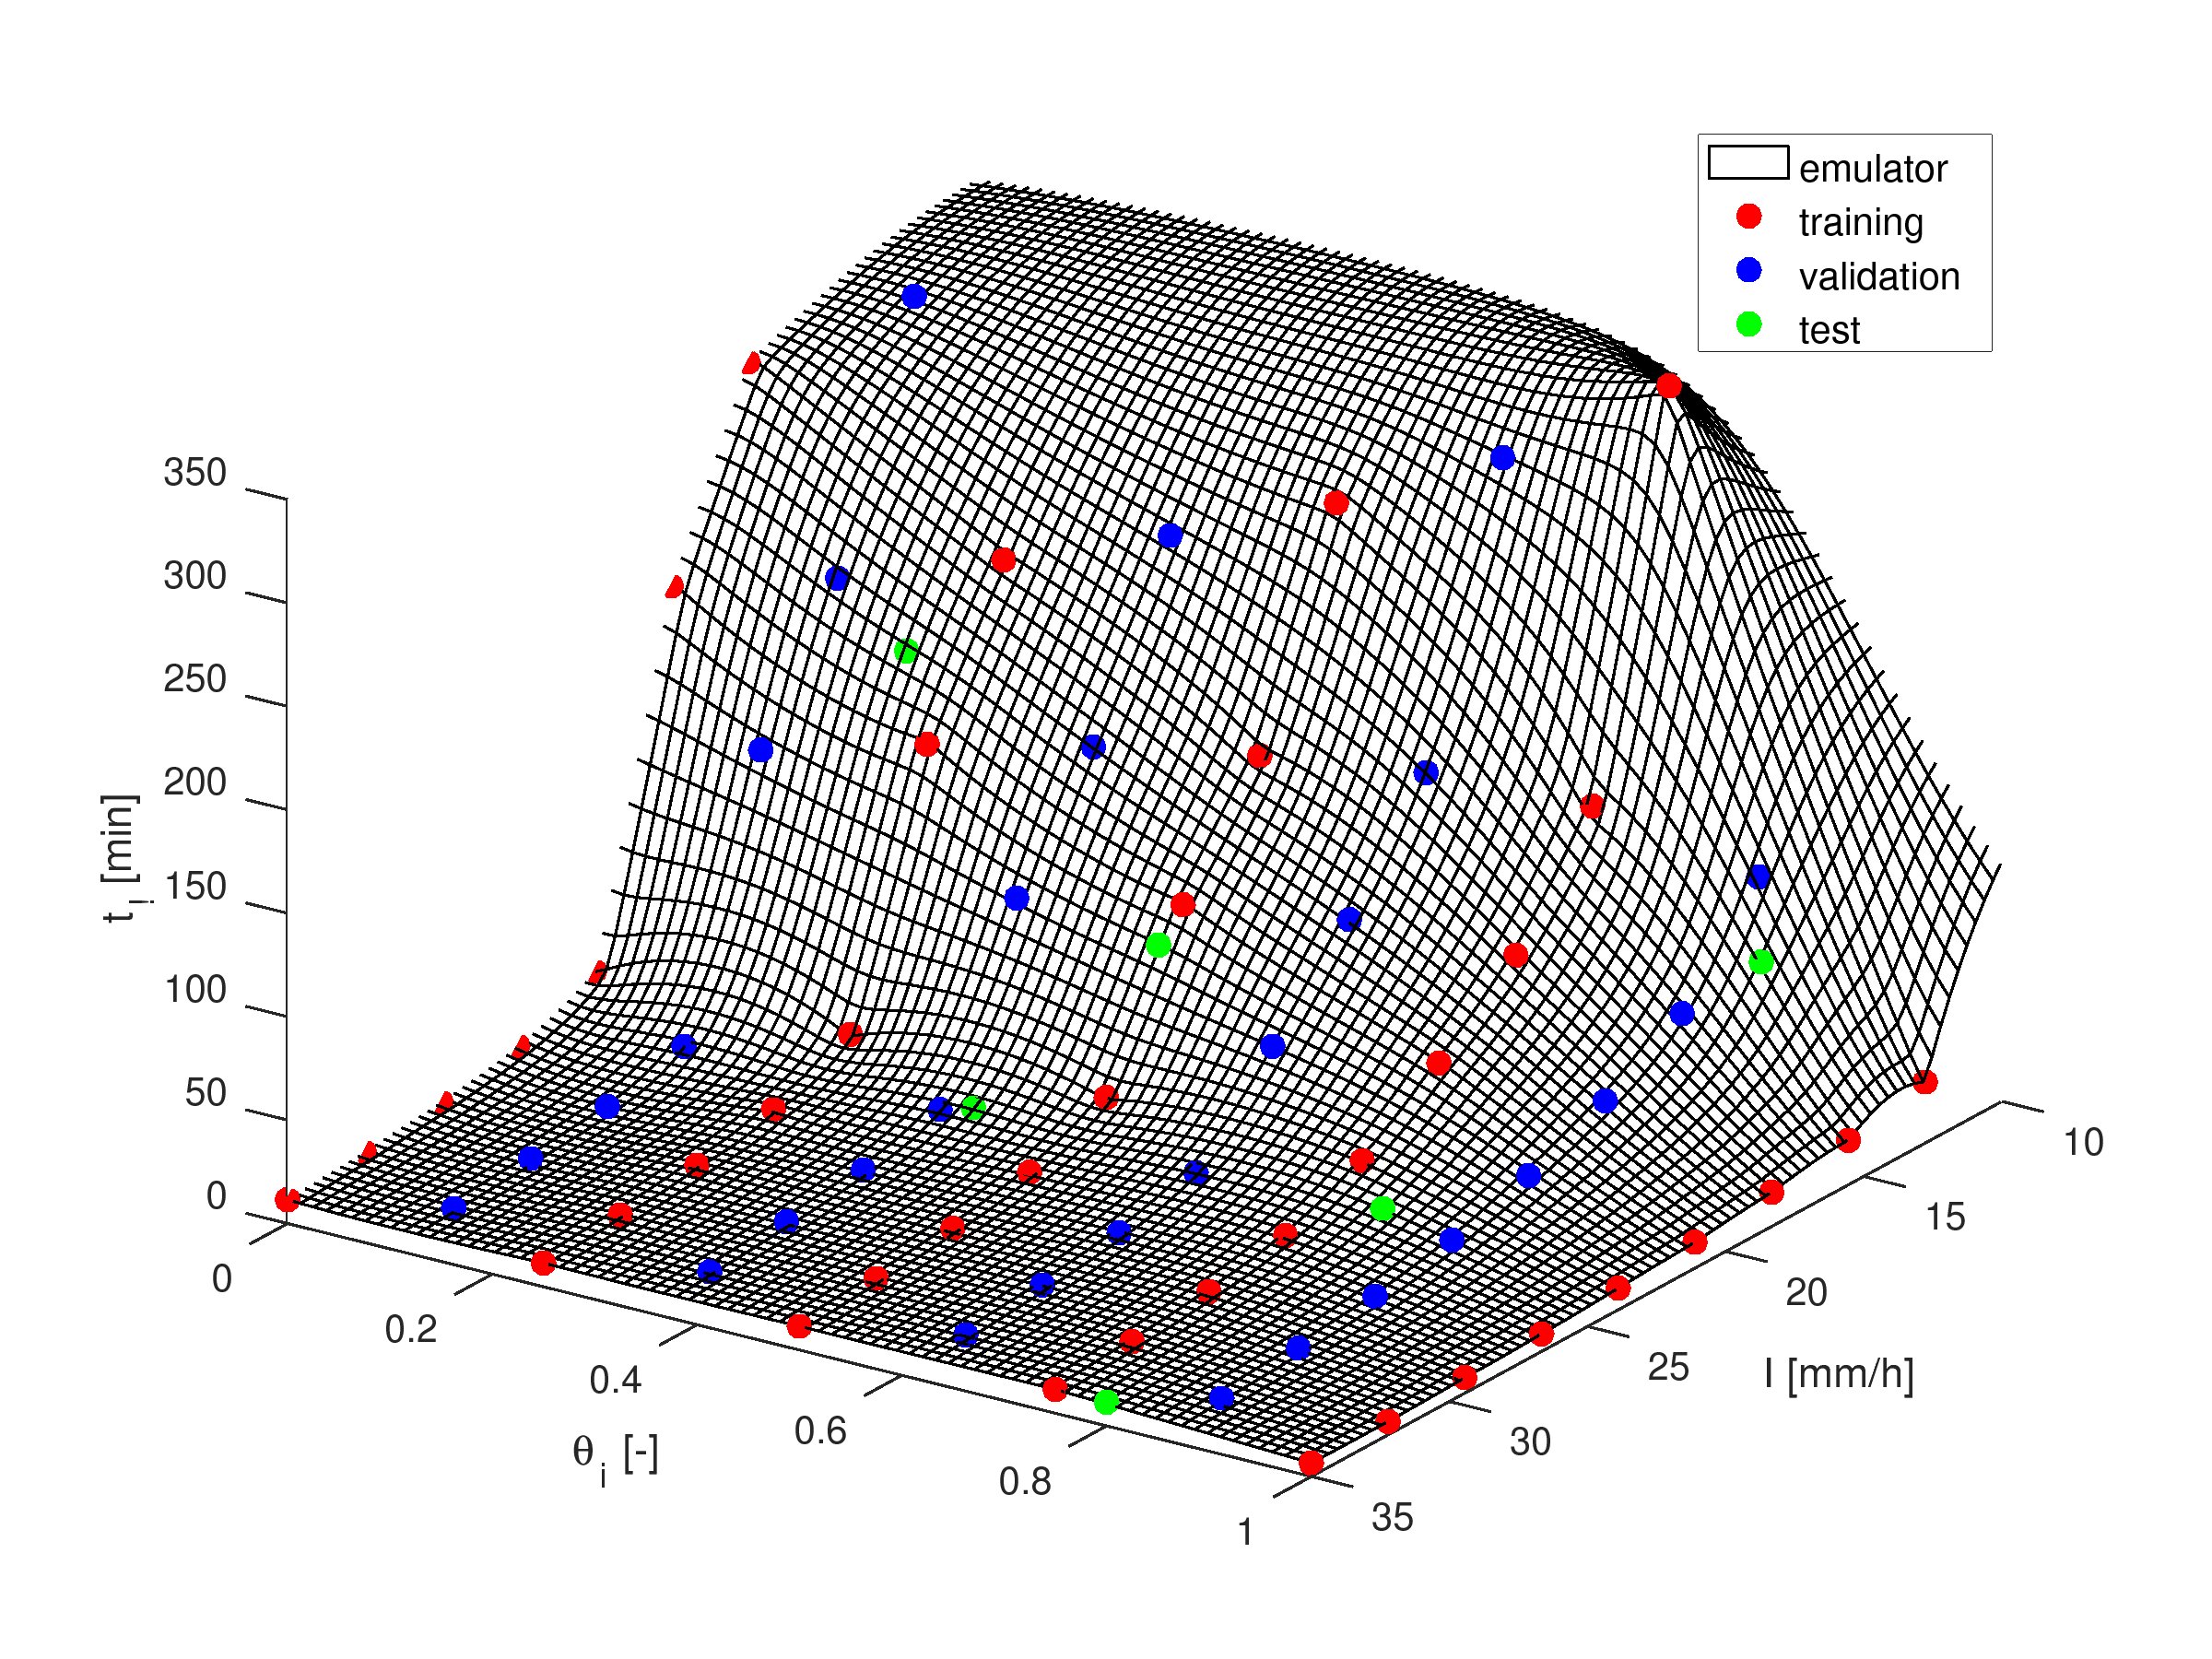
\includegraphics[width=0.8\textwidth]{img/emulator.png}
    }
    \only<2>{
    \centering
    \textbf{Test performance}\\
    \begin{table}[htpb]
      \centering
      \begin{tabular}{cc}
        \toprule
        MAE [min, \%] & RMSE [min]\\
        \midrule
        6.0, 5.9 & 4.0\\
        \bottomrule
      \end{tabular}
    \end{table}
    Duration one simulation: $\approx 30\,min$\\
    Duration one emulator-evaluation: $\approx 0.012\,s$
    \vfill
    \textbf{speedup factor}: $1.5 \cdot 10^5$
    }
  \end{frame}

% * The plot shows the times-to-threshold extracted from the simulations (the
%   red, blue and green points) as well as the predicted times-to-threshold for
%   regions where no simulation points are available
%   The red points were used to train the model the first time
% * The blue points were used to validate the model and were included for a
%   second training of the model
% * The green ones were taken for testing the model
% * The surface interpolates the training points: it computes the time-to-
%   threshold over the whole domain and was obtained using Gaussian Processes
% * Here I sum up the main results
% * Maximum absolute error on the validation dataset is 6 min, representing
%   a relative maximum absolute error of about 6%
% * The root mean squared error is 4 min
% * Here wee see how much faster is the proposed model in comparison with the
%   simulator

%%%%%%%%%%%%%%%%%%%%%%%%%%%%%%%%%%%%%%%%%%%%%%%%%%%%%%%%%%%%%%%%%%%%%%%%%%%%%%%%
% CONCLUSIONS
\section{Conclusion}
  \begin{frame}
    \frametitle{Conclusion \& Outlook}
    \begin{itemize}
    \itemsep0em
      \item Gaussian Processes can be a valid technique to build efficient
            surrogate models for the solution of specific tasks
            \begin{itemize}
            \itemsep0em
              \item Training of the model with \num{86} data points $\approx \SI{2.5}{\second}$
              \item Evaluation at one point $\approx \SI{0.012}{\s}$
            \end{itemize}
      \item For computationally expensive numerical models, like those solving
            the shallow water equation, this results in enormous speedups
      \item Despite the simplicity of the considered model, the methodology
            developed can be used for the construction of more complex ones
      \item The performance of more complex models (e.g. with more parameters)
            should be tested on a real case study
    \end{itemize}
    
  \end{frame}

%%%%%%%%%%%%%%%%%%%%%%%%%%%%%%%%%%%%%%%%%%%%%%%%%%%%%%%%%%%%%%%%%%%%%%%%%%%%%%%%
% FINAL SLIDE
{
\setbeamertemplate{footline}{} % no footer on title
\setbeamertemplate{background}{
\includegraphics[width=\paperwidth]{beamer_themes/background_slides_IAHR.png}}
  \begin{frame}
    \centering
    \vspace{0.2cm}
    \huge{\textbf{THANK YOU\\FOR YOUR ATTENTION}}\\
    \small
    \vspace{0.7cm}
    \url{https://bitbucket.org/binello7/fswof2d}
    \vspace{0.4cm}
    \url{https://bitbucket.org/binello7/master\_thesis}
  \end{frame}
}

\end{document}

